\documentclass{article}
\pagestyle{empty}
\usepackage{xcolor}
\usepackage{tikz}
\usetikzlibrary{calc, positioning, arrows.meta, fit}

\definecolor{problemred}{RGB}{140, 62, 84}

\tikzset{
  note/.style={align=left, font=\footnotesize},
  drift/.style={-Latex, thick},
  problemnote/.style={note, text=problemred},
  problemarrow/.style={drift, draw=problemred}
}

\begin{document}
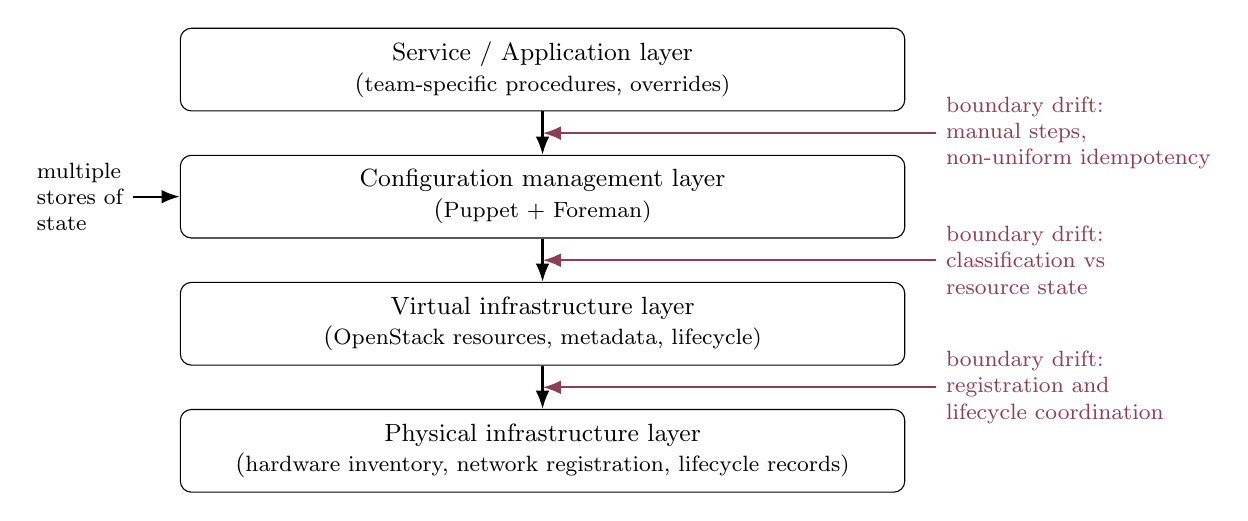
\begin{tikzpicture}[
    font=\small,
    box/.style={
        draw, rounded corners, align=center,
        minimum width=9.2cm, minimum height=1.05cm, inner sep=3pt
      },
    drift/.style={-Latex, thick},
    note/.style={align=left, font=\footnotesize},
    node distance=0.55cm
  ]

  \node[box] (svc) {Service / Application layer\\(\footnotesize team-specific procedures, overrides)};
  \node[box, below=of svc] (cm) {Configuration management layer\\(\footnotesize Puppet + Foreman)};
  \node[box, below=of cm] (cloud) {Virtual infrastructure layer\\(\footnotesize OpenStack resources, metadata, lifecycle)};
  \node[box, below=of cloud] (phys) {Physical infrastructure layer\\(\footnotesize hardware inventory, network registration, lifecycle records)};

  \coordinate (b1) at ($(svc.south)!0.5!(cm.north)$);
  \coordinate (b2) at ($(cm.south)!0.5!(cloud.north)$);
  \coordinate (b3) at ($(cloud.south)!0.5!(phys.north)$);

  \draw[drift] (svc.south) -- (cm.north);
  \draw[drift] (cm.south) -- (cloud.north);
  \draw[drift] (cloud.south) -- (phys.north);

  \node[problemnote, right=5cm of b1] (d1)
  {boundary drift:\\manual steps,\\non-uniform idempotency};
  \draw[problemarrow] (d1.west) -- (b1);

  \node[problemnote, right=5cm of b2] (d2)
  {boundary drift:\\classification vs\\resource state};
  \draw[problemarrow] (d2.west) -- (b2);

  \node[problemnote, right=5cm of b3] (d3)
  {boundary drift:\\registration and\\lifecycle coordination};
  \draw[problemarrow] (d3.west) -- (b3);

  \node[note, left=0.6cm of cm.west] (sot)
  {multiple\\stores of\\state};
  \draw[drift] (sot.east) -- (cm.west);

\end{tikzpicture}

\end{document}
